%; whizzy section -pdf xpdf -latex ./whizzypdfptex.sh
% latex beamer presentation.
% platex, latex-beamer $B$G%3%s%Q%$%k$9$k$3$H$rA[Dj!#(B 

%     Tokyo Debian Meeting resources
%     Copyright (C) 2008 Junichi Uekawa
%     Copyright (C) 2008 Nobuhiro Iwamatsu

%     This program is free software; you can redistribute it and/or modify
%     it under the terms of the GNU General Public License as published by
%     the Free Software Foundation; either version 2 of the License, or
%     (at your option) any later version.

%     This program is distributed in the hope that it will be useful,
%     but WITHOUT ANY WARRANTY; without even the implied warranty of
%     MERCHANTABILITY or FITNESS FOR A PARTICULAR PURPOSE.  See the
%     GNU General Public License for more details.

%     You should have received a copy of the GNU General Public License
%     along with this program; if not, write to the Free Software
%     Foundation, Inc., 51 Franklin St, Fifth Floor, Boston, MA  02110-1301 USA

\documentclass[cjk,dvipdfm,12pt]{beamer}
\usetheme{Tokyo}
\usepackage{ulem}
\usepackage{tabularx}

\usepackage{fancybox}
\usepackage{fancyvrb}   
\usepackage{float}

% commandline$B4D6-$rDj5A!#2hLLF~=PNO$K$D$$$F$O(Bcommandline$B4D6-(B
% $B$GI=5-$9$k(B
\newenvironment{commandline}%
{\VerbatimEnvironment
  \begin{Sbox}\begin{minipage}{0.9\hsize}\begin{fontsize}{7.3}{7.3} \begin{BVerbatim}}%
{\end{BVerbatim}\end{fontsize}\end{minipage}\end{Sbox}
  \setlength{\fboxsep}{8pt}
% start on a new paragraph

\vspace{6pt}% skip before
\fcolorbox{dancerdarkblue}{dancerlightblue}{\TheSbox}

\vspace{6pt}% skip after
}
%end of commandline

\definecolor{dancerdarkblue}{rgb}{0,0.08,0.45}
\definecolor{dancernormalblue}{rgb}{0.8,0.9,0.95}
\definecolor{dancerlightblue}{rgb}{0.8,0.95,1}


%  preview (shell-command (concat "evince " (replace-regexp-in-string "tex$" "pdf"(buffer-file-name)) "&"))
%  presentation (shell-command (concat "xpdf -fullscreen " (replace-regexp-in-string "tex$" "pdf"(buffer-file-name)) "&"))

%http://www.naney.org/diki/dk/hyperref.html
%$BF|K\8l(BEUC$B7O4D6-$N;~(B
\AtBeginDvi{\special{pdf:tounicode EUC-UCS2}}
%$B%7%U%H(BJIS$B7O4D6-$N;~(B
%\AtBeginDvi{\special{pdf:tounicode 90ms-RKSJ-UCS2}}

\title{$B%P!<%8%g%s4IM}%D!<%k$r;H$$(B Debian $B%Q%C%1!<%8$r4IM}$9$k(B}
\subtitle{Git $BJT(B}
\author{$B4d>>(B $B?.MN(B iwamatu@debian.or.jp\\IRC nick: iwamatsu}
\date{2008$BG/(B4$B7n(B19$BF|(B}
\logo{
\includegraphics[width=8cm]{image200607/openlogo-light.eps}}


% $B4V$N%?%$%H%k%Z!<%8MQ(B
\newcommand{\emtext}[1]{
\begin{frame}{}
 
\begin{minipage}{0.55\hsize}
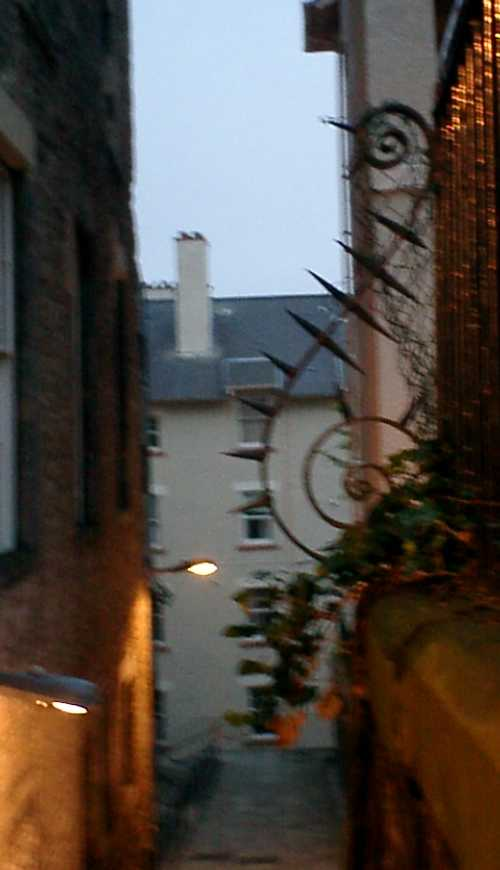
\includegraphics[width=1\hsize]{image200707/gurutitle.jpg}
\end{minipage}
\begin{minipage}{0.39\hsize}
 {\Huge #1
 }
\end{minipage}
\end{frame}
}

% $B;0BrLdBjMQ(B
\newcounter{santakucounter}
\newcommand{\santaku}[5]{%
\addtocounter{santakucounter}{1}
\frame{\frametitle{$BLdBj(B\arabic{santakucounter}. #1}
%$BLdBj(B\arabic{santakucounter}. #1
\begin{minipage}[t]{0.8\hsize}
 \begin{itemize}
 \item
      \begin{minipage}{0.2\hsize}
      
\includegraphics[width=0.9\hsize]{image200703/janken-A.png}\end{minipage} 
       \begin{minipage}{0.6\hsize}
       A #2\end{minipage}\\
 \item
      \begin{minipage}{0.2\hsize}
      
\includegraphics[width=0.9\hsize]{image200703/janken-B.png}\end{minipage} 
       \begin{minipage}{0.6\hsize}
       B #3\end{minipage}\\
 \item
      \begin{minipage}{0.2\hsize}
      
\includegraphics[width=0.9\hsize]{image200703/janken-C.png}\end{minipage} 
       \begin{minipage}{0.6\hsize}
       C #4\end{minipage}\\
 \end{itemize}
\end{minipage}
}
\frame{\frametitle{$BLdBj(B\arabic{santakucounter}. #1}
%$BLdBj(B\arabic{santakucounter}. #1
\begin{minipage}[t]{0.8\hsize}
\begin{itemize}
 \item
      \begin{minipage}{0.2\hsize}
      
\includegraphics[width=0.9\hsize]{image200703/janken-A.png}\end{minipage} 
       \begin{minipage}{0.6\hsize}
       A #2\end{minipage}\\
 \item
      \begin{minipage}{0.2\hsize}
      
\includegraphics[width=0.9\hsize]{image200703/janken-B.png}\end{minipage} 
       \begin{minipage}{0.6\hsize}
       B #3\end{minipage}\\
 \item
      \begin{minipage}{0.2\hsize}
      
\includegraphics[width=0.9\hsize]{image200703/janken-C.png}\end{minipage} 
       \begin{minipage}{0.6\hsize}
       C #4\end{minipage}\\
\end{itemize}
\end{minipage}
\begin{minipage}[t]{0.15\hsize}
$BEz$($O(B:

\vspace{1cm}

  {\huge \hspace{1cm}#5}
  \hspace{-6cm}\includegraphics[width=4cm]{image200703/janken-#5.png}
 \end{minipage}}
}

\begin{document}

\frame{\titlepage{}}


\section{$B$O$8$a$K(B}

\begin{frame}{$B$J$<%Q%C%1!<%8$b(BVCS$B$G4IM}$9$k$N$+(B}
\begin{itemize}
  \item $B0[$J$k%P!<%8%g%s$N%Q%C%1!<%8$r4IM}$9$k$3$H$,$G$-$k!#(B
  \item $B%A!<%`$G$N3+H/BN@)$rMF0W$K9=C[$G$-$k!#(B
  \item $B%"%C%W%9%H%j!<%`$H$NO"7H(B
\end{itemize}
\end{frame}

\begin{frame}{Debian $B$G;HMQ2DG=$J(B VCS}
\begin{center}
2008$BG/(B4$B7n$N;~E@$G$N(B Debian $B$GMxMQ2DG=$J(B VCS
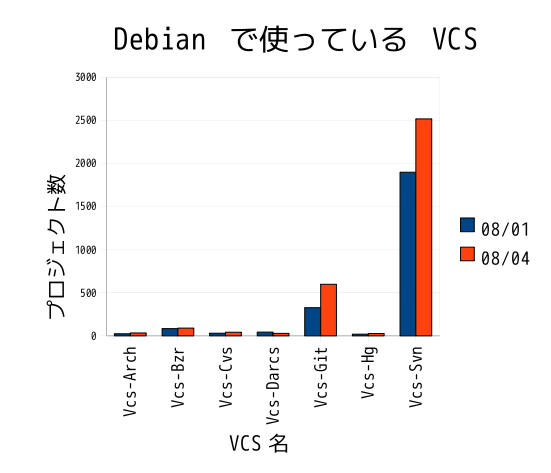
\includegraphics[width=1.0\hsize]{image200804/debian-vcs-200804.png}
\end{center}
\end{frame}


\begin{frame}{git-buildpackage}

\begin{itemize}

\item git-buildpackage 

$B%Q%C%1!<%8$r:n@.$9$k(B \\
\item git-dch 

Git $B$N%3%_%C%H%m%0$+$i(B Debian Changelog $B$r:n@.$9$k!#(B\\
\item git-import-dsc 

$B4{B8$N(B Debian Package $B$r(BGit$B$K%$%s%]!<%H$9$k!#(B\\
\item git-import-orig 

$B%"%C%W%9%H%j!<%`$+$i%j%j!<%9$5$l$?%=!<%9%3!<%I$r(BGit$B$K%$%s%]!<%H$9$k!#(B\\

\end{itemize}
\end{frame}

\begin{frame}{Git$B$N4JC1$J;H$$J}(B}
\begin{center}
SD 2008$BG/(B 4$B7n9f(B $B$rGc$&$H$$$$$h!#(B
%\includegraphics[width=0.5\hsize]{image200804/1208082175384ed79.jpg}
\end{center}
\end{frame}

\begin{frame}{Git$B$N4JC1$J;H$$J}(B}
   \begin{itemize}
\item git clone

$B%j%b!<%H%j%]%8%H%j$+$i>pJs$r<hF@$7!"%m!<%+%k%j%]%8%H%j$r:n@.$9$k!#(B\

\item git init

$B%m!<%+%k%j%]%8%H%j$r:n@.$9$k!#(B\\
\item git add

$B%m!<%+%k%j%]%8%H%j$N%-%c%C%7%e(B(index)$B$K4IM}BP>]$N%U%!%$%k$rDI2C$9$k!#(B\\
\item git commit

$B%m!<%+%k%j%]%8%H%j$KJQ99$rH?1G$9$k!#(B\\
\item git rm

$B%m!<%+%k%j%]%8%H%j$+$i4IM}BP>]%U%!%$%k$r:o=|$9$k!#(B\\
\item git diff

\end{itemize}
\end{frame}

\begin{frame}{Git$B$N4JC1$J;H$$J}(B}
   \begin{itemize}
   \item git diff

$B:9J,$r<hF@$9$k!#(B\\
\item git branch

$B%V%i%s%A$r:n@.$9$k!#(B\\
\item git checkout

$B:n@.$7$?%V%i%s%A$r%A%'%C%/%"%&%H$9$k!#(B\\
\item git format-patch

$B%Q%C%A$r:n@.$9$k!#(B\\

\item git pull

$B%j%b!<%H%j%]%8%H%j$+$iJQ99$r<hF@$9$k!#(B\\

\item git push

$B%j%b!<%H%j%]%8%H%j$XJQ99$rH?1G$9$k!#(B\\
\end{itemize}
\end{frame}

\emtext{$B%Q%C%1!<%82=$5$l$F$$$k$b$N$r(B Git $B$G4IM}$9$k(B}

\begin{frame}[containsverbatim]{Debian Package $B>pJs$N<h$j9~$_(B}

\begin{minipage}{0.5\hsize}

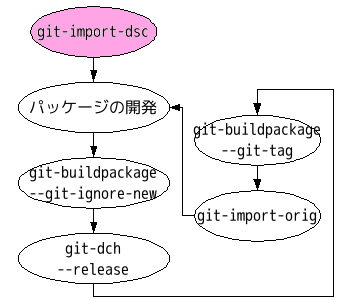
\includegraphics[width=1.0\hsize]{image200804/test1-1.png}
\end{minipage} 
\begin{minipage}{0.45\hsize}
\begin{commandline}
$ git-import-dsc ../isight-firmware-
tools_1\.0.2-1.dsc
Upstream version: 1.0.2
Debian version: 1
No git repository found, creating one.
Initialized empty Git repository in \
.git/
Everything imported under isight-firm\
ware-tools
$ ls
isight-firmware-tools
$ cd isight-firmware-tools
$ git branch
* master
  upstream
\end{commandline}
\end{minipage}
\end{frame}


\begin{frame}[containsverbatim]{$B%$%s%]!<%H;~$N%m%0(B}

\begin{minipage}{0.5\hsize}

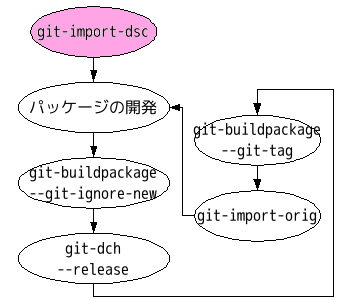
\includegraphics[width=1.0\hsize]{image200804/test1-1.png}
\end{minipage} 
\begin{minipage}{0.45\hsize}
\begin{commandline}
$ git log
commit 9c3669a233afe69d7be2aa8ad199\
5e6b19c841aa
Author: Nobuhiro Iwamatsu <iwamatsu@\
nigauri.org>
Date:   Sun Apr 6 21:48:40 2008 +0900

    Imported Debian patch 1.0.2-1
$ git tag
debian/1.0.2-1
upstream/1.0.2
\end{commandline}
\end{minipage}
\end{frame}
%%

\begin{frame}[containsverbatim]{$B%=!<%9%3!<%I$rJQ99$7!"=$@5$r4IM}$9$k(B}

\begin{minipage}{0.5\hsize}

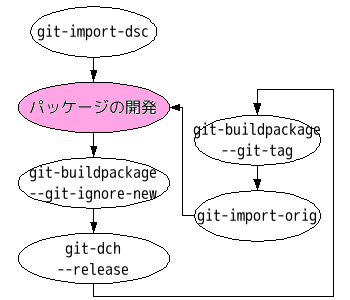
\includegraphics[width=1.0\hsize]{image200804/test1-2.png}
\end{minipage} 
\begin{minipage}{0.45\hsize}

\begin{commandline}
$ dpatch-edit-patch 05_change_ift-load \
_install_dir
... $B$$$m$$$m=$@5(B ...
$ exit
$ vi debian/patches/00list
$ git add debian/patches/05chage_ift\
-load_install_dir.dpatch
$ git commit -s debian/patches/00list\
 debian/patches/05_chage_ift-load_inst\
all_dir.dpatch
/* $B%(%G%#%?$,5/F0$9$k$N$G!"%3%_%C%H%m%0$r5-=R(B */

Change ift-load install dir.
    
Signed-off-by: Nobuhiro Iwamatsu \
<iwamatsu@nigauri.org>

$ git log
commit c9865153ae1949956fdfe3827c0da9b3\
6c2f0ddb
Author: Nobuhiro Iwamatsu <iwamatsu@niga\
uri.org>
Date:   Sun Apr 6 21:23:20 2008 +0900

    Change ift-load install dir.
    
    Signed-off-by: Nobuhiro Iwamatsu <iwa\
matsu@nigauri.org>
\end{commandline}
\end{minipage}
\end{frame}

\begin{frame}[containsverbatim]{git-buildpackage $B$r;H$C$?(BDebian $B%Q%C%1!<%8$N:n@.(B}

\begin{minipage}{0.5\hsize}

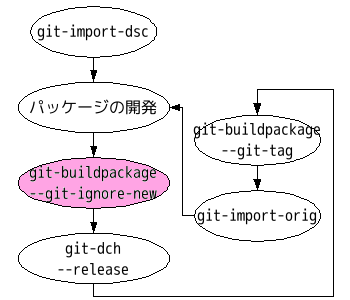
\includegraphics[width=1.0\hsize]{image200804/test1-3.png}
\end{minipage} 
\begin{minipage}{0.45\hsize}

\begin{commandline}
$ git-buildpackage --git-ignore-new\
 -us -uc
\end{commandline}

\end{minipage}
\end{frame}

%%

\begin{frame}[containsverbatim]{$B%Q%C%1!<%8$r%j%j!<%9$9$k(B}
\begin{minipage}{0.5\hsize}
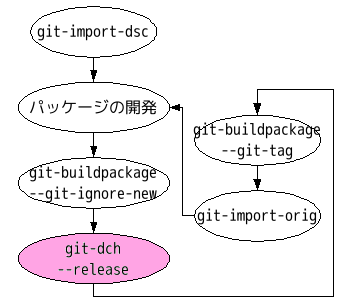
\includegraphics[width=1.0\hsize]{image200804/test1-4.png}
\end{minipage} 
\begin{minipage}{0.45\hsize}
\begin{commandline}
$ git-dch --release
/* $B%(%G%#%?$,N)$A>e$,$j!"(BDebian Changelog 
   $B$rF~NO$9$k(B  */
\end{commandline}
\end{minipage}
\end{frame}

\begin{frame}[containsverbatim]{$B%j%j!<%9%?%0$rIU$1$F!"%Q%C%1!<%8$r:n@.$9$k(B}
\begin{minipage}{0.5\hsize}
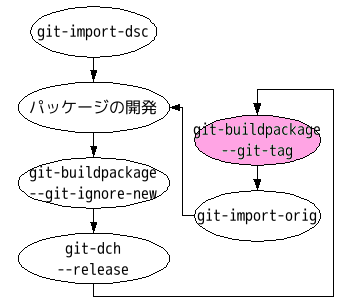
\includegraphics[width=1.0\hsize]{image200804/test1-5.png}
\end{minipage} 
\begin{minipage}{0.45\hsize}
\begin{commandline}
$ git-buildpackage --git-ignore-new\
 --git-tag
$ git tag
debian/1.0.2-1
debian/1.0.2-2
upstream/1.0.2
\end{commandline}
\end{minipage}
\end{frame}

\begin{frame}[containsverbatim]{$B?7$7$$%P!<%8%g%s$K$9$k(B}
\begin{minipage}{0.5\hsize}
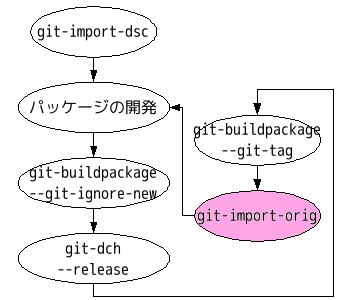
\includegraphics[width=1.0\hsize]{image200804/test1-6.png}
\end{minipage} 
\begin{minipage}{0.45\hsize}
\begin{commandline}
$ git-import-orig /tmp/isight-\
firmware-tools-1.2.tar.gz
Upstream version is 1.2.0
Importing '/tmp/isight-firmware\
-tools-1.2.tar.gz' to branch 'upstream'...
Switched to branch "upstream"
rm 'isight.rules.in'
rm 'po/fr_FR.po'
Created commit f5c85da: Imported\
 Upstream version 1.2.0
 33 files changed, 4434 insertio\
ns(+), 1332 deletions(-)

.......<snip>

 src/udev.c                      \
       |  164 +++
 33 files changed, 4434 insertion\
s(+), 1332 deletions(-)
 rename po/{fr_FR.po => fr.po} (66%)
 create mode 100644 src/50-isight-\
firmware.fdi
\end{commandline}
\end{minipage}
\end{frame}

\begin{frame}[containsverbatim]{$B?7$7$$%P!<%8%g%s$K$9$k(B}
\begin{minipage}{0.5\hsize}
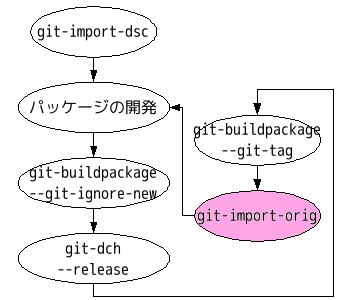
\includegraphics[width=1.0\hsize]{image200804/test1-6.png}
\end{minipage} 
\begin{minipage}{0.45\hsize}
\begin{commandline}
 create mode 100644 src/callout.c
 create mode 100644 src/isight-firm\
ware.fdi
 rename isight.rules.in => src/isigh\
t.rules.in (100%)
 create mode 100644 src/load.h
 create mode 100644 src/udev.c
Succesfully merged version 1.2 of \
/home/iwamatsu/Desktop/isight-firmwar\
e-tools-1.2.tar.gz into .
$ git branch
debian/1.0.2-1
debian/1.0.2-2
upstream/1.0.2
upstream/1.2
$ cat debian/changelog
isight-firmware-tools (1.2-1) unstable;\
 urgency=low

  * New Upstream Version

 -- Nobuhiro Iwamatsu <iwamatsu@\
nigauri.org>  Fri, 11 Apr 2008 17:18:23 +0900

\end{commandline}
\end{minipage}
\end{frame}

\begin{frame}[containsverbatim]{$B?7$?$K%Q%C%1!<%82=$9$k>l9g(B}
\begin{minipage}{0.5\hsize}
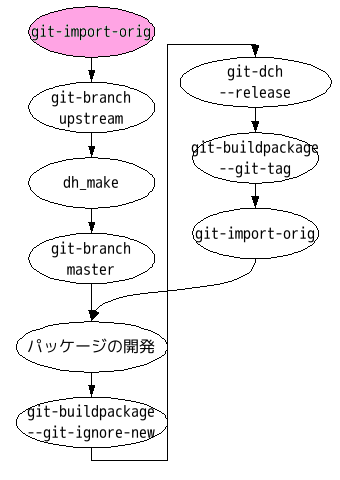
\includegraphics[width=1.0\hsize]{image200804/test-1.png}
\end{minipage} 
\begin{minipage}{0.45\hsize}
\begin{commandline}
$ mkdir isight-firmware-loader-1.2
$ cd isight-firmware-tools-1.2
$ git-init
$ git-import-orig -u 1.2 \
/tmp/isight-firmware-tools-1.2.tar.gz
Upstream version is 1.2
Initial import of '/tmp/isight-\
firmware-tools-1.2.tar.gz' ...
Succesfully merged version 1.2 \
of /tmp/isight-firmware-tools-1.2.tar.gz into .
$ git log
commit 9bf014aee2f834576f8f03d67\
ab66e8c85726832
Author: Nobuhiro Iwamatsu <iwamat\
su@nigauri.org>
Date:   Tue Apr 8 21:42:55 2008 +0900

    Imported Upstream version 1.2
$ git branch
* master
  upstream
$ git tag
upstream/1.2
$ git branch upsteam
$ dh_make
$ git branch master
\end{commandline}

\end{minipage}
\end{frame}


\begin{frame}[containsverbatim]{$B?7$?$K%Q%C%1!<%82=$9$k>l9g(B}
\begin{minipage}{0.5\hsize}
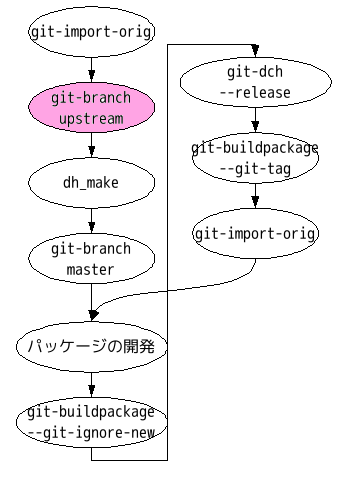
\includegraphics[width=1.0\hsize]{image200804/test-2.png}
\end{minipage} 
\begin{minipage}{0.45\hsize}
\begin{commandline}
$ mkdir isight-firmware-loader-1.2
$ cd isight-firmware-tools-1.2
$ git-init
$ git-import-orig -u 1.2 \
/tmp/isight-firmware-tools-1.2.tar.gz
Upstream version is 1.2
Initial import of '/tmp/isight-\
firmware-tools-1.2.tar.gz' ...
Succesfully merged version 1.2 \
of /tmp/isight-firmware-tools-1.2.tar.gz into .
$ git log
commit 9bf014aee2f834576f8f03d67\
ab66e8c85726832
Author: Nobuhiro Iwamatsu <iwamat\
su@nigauri.org>
Date:   Tue Apr 8 21:42:55 2008 +0900

    Imported Upstream version 1.2
$ git branch
* master
  upstream
$ git tag
upstream/1.2
$ git branch upsteam
$ dh_make
$ git branch master
\end{commandline}

\end{minipage}
\end{frame}


\begin{frame}[containsverbatim]{$B?7$?$K%Q%C%1!<%82=$9$k>l9g(B}
\begin{minipage}{0.5\hsize}
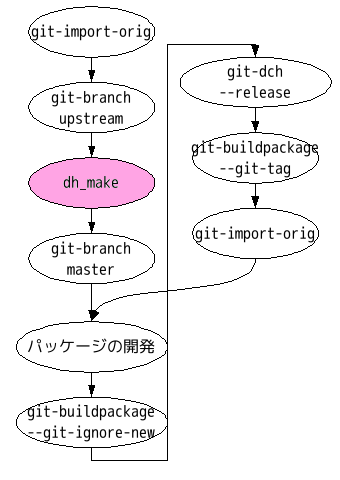
\includegraphics[width=1.0\hsize]{image200804/test-3.png}
\end{minipage} 
\begin{minipage}{0.45\hsize}
\begin{commandline}
$ mkdir isight-firmware-loader-1.2
$ cd isight-firmware-tools-1.2
$ git-init
$ git-import-orig -u 1.2 \
/tmp/isight-firmware-tools-1.2.tar.gz
Upstream version is 1.2
Initial import of '/tmp/isight-\
firmware-tools-1.2.tar.gz' ...
Succesfully merged version 1.2 \
of /tmp/isight-firmware-tools-1.2.tar.gz into .
$ git log
commit 9bf014aee2f834576f8f03d67\
ab66e8c85726832
Author: Nobuhiro Iwamatsu <iwamat\
su@nigauri.org>
Date:   Tue Apr 8 21:42:55 2008 +0900

    Imported Upstream version 1.2
$ git branch
* master
  upstream
$ git tag
upstream/1.2
$ git branch upsteam
$ dh_make
$ git branch master
\end{commandline}

\end{minipage}
\end{frame}



\begin{frame}[containsverbatim]{$B?7$?$K%Q%C%1!<%82=$9$k>l9g(B}
\begin{minipage}{0.5\hsize}
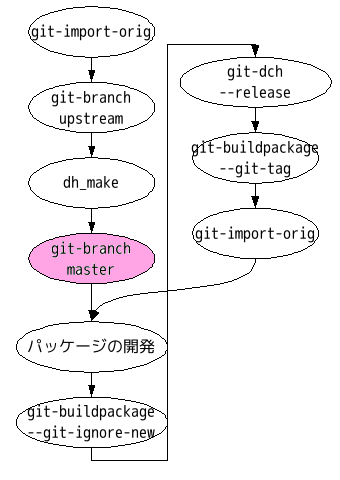
\includegraphics[width=1.0\hsize]{image200804/test-4.png}
\end{minipage} 
\begin{minipage}{0.45\hsize}
\begin{commandline}
$ mkdir isight-firmware-loader-1.2
$ cd isight-firmware-tools-1.2
$ git-init
$ git-import-orig -u 1.2 \
/tmp/isight-firmware-tools-1.2.tar.gz
Upstream version is 1.2
Initial import of '/tmp/isight-\
firmware-tools-1.2.tar.gz' ...
Succesfully merged version 1.2 \
of /tmp/isight-firmware-tools-1.2.tar.gz into .
$ git log
commit 9bf014aee2f834576f8f03d67\
ab66e8c85726832
Author: Nobuhiro Iwamatsu <iwamat\
su@nigauri.org>
Date:   Tue Apr 8 21:42:55 2008 +0900

    Imported Upstream version 1.2
$ git branch
* master
  upstream
$ git tag
upstream/1.2
$ git branch upsteam
$ dh_make
$ git branch master
\end{commandline}

\end{minipage}
\end{frame}



\section{$B%"%C%W%9%H%j!<%`$N(B VCS $B$HIU$-9g$&(B}
\emtext{$B%"%C%W%9%H%j!<%`$N(B VCS $B$HIU$-9g$&(B}

\begin{frame}[containsverbatim]{$B%"%C%W%9%H%j!<%`$N(B VCS $B$HIU$-9g$&(B}

\begin{itemize}
\item $B%"%C%W%9%H%j!<%`$,(B VCS $B$r;H$C$F$$$k(B
\item $B<+J,$H$O<qL#$N0[$J$k(BVCS$B$r;H$C$F$$$k(B
\item Debian Package $B%a%s%F%J$H$7$F$I$N$h$&$KIU$-9g$($P$$$$$N$+(B
\end{itemize}
\end{frame}


\begin{frame}[containsverbatim]{$B%"%C%W%9%H%j!<%`$,(B Subversion $B$r;H$C$F$$$k>l9g(B}

\begin{itemize}
\item $B<+J,$b(B Subversion$B$r;H$C$F$$$k>l9g(B

svn-buildpackage$B!!$GO"7H$9$k$3$H$,2DG=(B

\item Git $B;H$$$?$$(B

git-svn $B$G(B Git $B%j%]%8%H%j7A<0$KJQ49$7$F$+$i;H$&(B

\end{itemize}
\end{frame}


\begin{frame}[containsverbatim]{SVN $B$N%j%]%8%H%j$+$i!!(BGit $B$N%j%]%8%H%j$XJQ49$9$k(B}

\begin{minipage}{0.48\hsize}
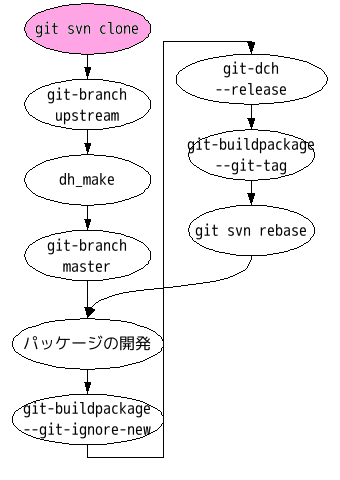
\includegraphics[width=1.0\hsize]{image200804/test2-1.png}
\end{minipage} 
\begin{minipage}{0.45\hsize}
\begin{commandline}
$ mkdir test
$ git svn clone svn://test/trunk test-0.0.1
\end{commandline}
\end{minipage} 
\end{frame}

\begin{frame}[containsverbatim]{$B<hF@$7$?%3!<%I$r85$K(B Debian Package $B$r:n@.$9$k(B}
\begin{minipage}{0.48\hsize}
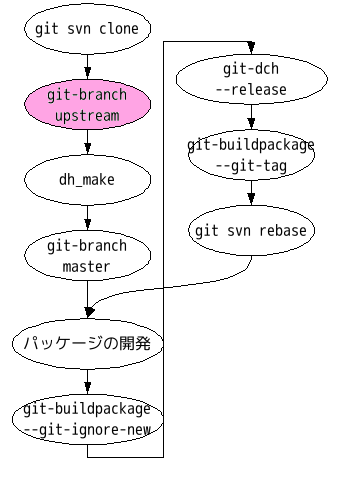
\includegraphics[width=1.0\hsize]{image200804/test2-2.png}
\end{minipage} 
\begin{minipage}{0.45\hsize}
\begin{commandline}
$ git branch
master
$ git branch upstream
$ git checkout upstream
$ git tag upstream/0.0.1
$ dh_make --createorig
$ git branch master
-- Debian Package $BMQ$N%U%!%$%k:n@.$J$I$r9T$&(B
$ git-buildpackage -us -uc \
--git-ignore-new
$ debuild clean
$ git add debian
$ git commit -a
$ git-buildpackage -us -uc \
--git-ignore-new --git-tag
\end{commandline}
\end{minipage} 
\end{frame}


\begin{frame}[containsverbatim]{Subversion $B%j%]%8%H%j$N>pJs$r<hF@$9$k(B}
\begin{minipage}{0.48\hsize}
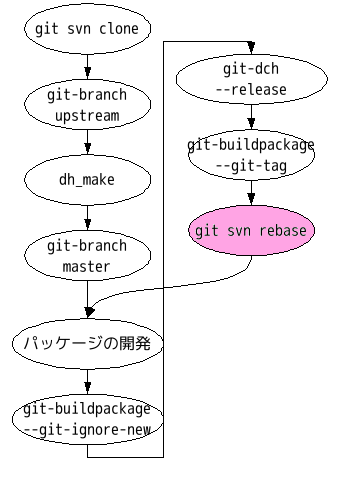
\includegraphics[width=1.0\hsize]{image200804/test2-3.png}
\end{minipage} 
\begin{minipage}{0.45\hsize}
\begin{commandline}
$ git checkout upstream
$ git svn rebase
\end{commandline}
\end{minipage} 
\end{frame}


\begin{frame}[containsverbatim]{$B$9$G$K$"$k%Q%C%1!<%8$H(B Git $B%j%]%8%H%j$r85$K:n@.$9$k(B}

\begin{minipage}{0.48\hsize}
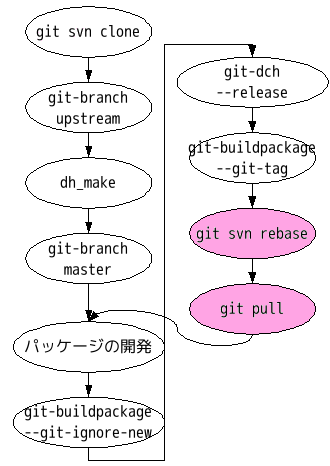
\includegraphics[width=1.0\hsize]{image200804/test3-1.png}
\end{minipage} 
\begin{minipage}{0.45\hsize}
\begin{commandline}

$ git svn clone svn://svn.berlios.de/\
linux-uvc/linux-uvc/trunk\
 linux-uvc.git
$ git import-dsc  ../../../debian/\
linux-uvc_0.1.0.svn193-2.dsc
$ cd linux-uvc
$ git branch
* master
  upstream
$ git tag
debian/0.1.0.svn193-2
upstream/0.1.0.svn193
$ git checkout upstream
$ git pull ../linux-uvc.git/
$ git tag upstream/0.1.0.svn201
$ git checkout master
$ dch -v 0.1.0.svn201
$ git-buildpackage -us -uc \
--git-ignore-new
$ debuild clean
$ git commit -a
$ git-buildpackage -us -us \
--git-ignore-new --git-tag
\end{commandline}
\end{minipage} 
\end{frame}

\begin{frame}{git-svn + git-buildpaclage$B$NLdBjE@(B}
\begin{itemize}
\item Git$B$NMxE@$,$&$^$/MxMQ$G$-$J$$(B

  git svn rebase $B$r;H$C$F$N3+H/J}K!$,ITL@(B
\item git tag $B$,$a$s$I$&!#(B

  Subversion $B$N%j%j!<%9%?%0$r$&$^$/3hMQ$G$-$J$$$+!#(B
\end{itemize}
\end{frame}

\end{document}

;;; Local Variables: ***
;;; outline-regexp: "\\([ 	]*\\\\\\(documentstyle\\|documentclass\\|emtext\\|section\\|begin{frame}\\)\\*?[ 	]*[[{]\\|[]+\\)" ***
;;; End: ***
